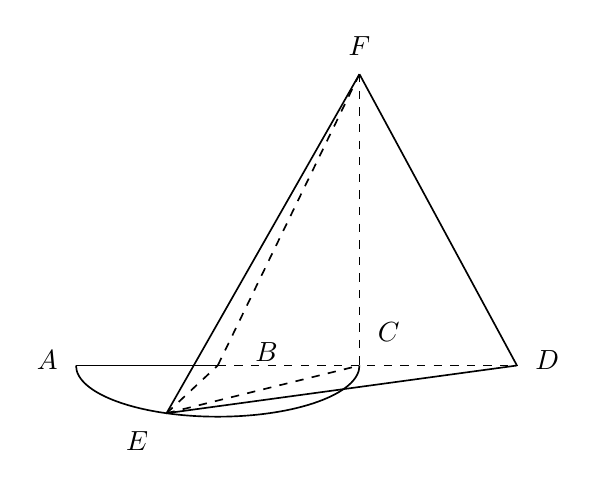
\begin{tikzpicture}[x=1cm,y=1cm,line width=0.6pt,font=\normalsize]
\coordinate (A) at (-3.2,0);
\coordinate (B) at (-1.4,0);
\coordinate (C) at (0.4,0);
\coordinate (D) at (2.4,0);
\coordinate (E) at (-2.0500000000,-0.6061398175);
\coordinate (F) at (0.4000000000,3.7000000000);
% base AD: solid left part, dashed right part
\draw[solid] (A)--(B);
\draw[dashed] (B)--(D);
% semicircle AEC: half ellipse with diameter AC, E at bottom
\draw[solid] (A) arc (180:360:1.8 and 0.65);
% pyramid edges
\draw[solid] (F)--(E);
\draw[solid] (F)--(D);
\draw[dashed] (F)--(C);
\draw[dashed] (F)--(B);
% base triangle BED part
\draw[solid] (E)--(D);

\draw[dashed] (E)--(C);
% labels with clearance
\node[left,xshift=-3pt,yshift=2.0pt] at (A) {$A$};
\node[right,xshift=10pt,yshift=5pt] at (B) {$B$};
\node[above right=3pt,yshift=2pt] at (C) {$C$};
\node[right,xshift=3pt,yshift=2.0pt] at (D) {$D$};
\node[below left,xshift=-3pt,yshift=-3pt] at (E) {$E$};
\node[above,yshift=3pt] at (F) {$F$};
\draw[dashed] (E)--(B);
\end{tikzpicture}
